
\paragraph{Section Overview}
In this section, we ask what current Neural Computer (NC) prototypes have already shown, what still prevents them from becoming usable or general-purpose runtimes, and why neither current world models~\citep{ha2018world,openai2024sora,polyak2024movie,deepmind_veo_2025} nor AI agents~\citep{hong2023metagpt,claudeComputerTool,zhuge2026ai} yet amount to this emerging machine form.
We then contrast NCs with conventional computers, clarifying that they are not a smarter layer on top of the existing stack, and define their mature general-purpose form, namely Completely Neural Computers (CNCs).
Finally, we outline a roadmap toward CNCs, relate NCs to other system objects, and close with several remarks on NCs.

\subsection{From Neural Computers to Completely Neural Computers}

\paragraph{Current Status of NCs}
Our CLI and GUI-based neural computers already show that early runtime primitives can be learned with measurable interface fidelity. In terminal environments, OCR-based text fidelity is already measurable (\Cref{tab:cligen-ocr}); in GUI settings, explicit visual supervision yields strong local cursor control (\Cref{tab:cursor-loss}); and in GUIWorld, aligned goal-directed data clearly outperforms much larger random exploration (\Cref{tab:gui-data-quality}). Taken together, these results suggest that current NCs already support early runtime primitives, especially I/O alignment and short-horizon control, while stable reuse and general-purpose execution remain out of reach.
This does not mean that current prototypes are already close to CNCs; it means that the outline of a distinct machine form has begun to emerge at prototype scale.

However, the current video-based prototypes are only early NC instantiations: if NCs are to mature into general-purpose runtimes, they must go well beyond basic I/O and short-term execution.
At the formal level, this ultimately requires Turing completeness~\citep{Goedel:31,Church:35,turing1936computable,siegelmann1992computational}, universal programmability~\citep{von1993first,wilkes1981best}, and behavior consistency unless explicitly reprogrammed~\citep{queloz2025explainability}.
Before those conditions are met in full, progress is better read through practical acceptance lenses: routine reuse, execution consistency, and explicit update governance.
These lenses matter because the immediate question is not whether CNCs have already been achieved, but whether NCs are beginning to behave more like usable runtimes than isolated demonstrations.
For example, once an incident-response routine has been installed, the system should reuse it on later alerts rather than rediscovering the procedure from scratch each time; and if its behavior changes, that change should be attributable to an explicit update rather than ordinary execution.
In practice, this reduces to three acceptance lenses: install--reuse, execution consistency, and update governance, which together offer a more useful view of current NC progress than the full CNC definition alone.

While certain sequential neural architectures are Turing complete~\citep{siegelmann1992computational,perez2021attention} in principle, turning a trained instance into a reliably programmable runtime remains challenging.
Preliminary attempts, including Neural Virtual Machine~\citep{katz2019programmable} and NeuroLISP~\citep{davis2022neurolisp}, have been explored.
Furthermore, ensuring stable behavior over long temporal horizons remains an open problem in neural systems~\citep{kirkpatrick2017overcoming,calanzonelogically}. 
Section~\ref{sec:roadmap} provides a more detailed discussion of these requirements. 
To the best of our knowledge, existing works on world models lack an analysis of the computability class of the learned models.
See Section~\ref{sec:relations} for more discussion between NCs and other system objects, including world models and AI agents.

\begin{table}[h]
  \centering
  \small
  \rowcolors{2}{tablewarmrow}{white}
  \caption{Four system objects compared at a common systems level.}
  \label{tab:system-objects}
  \setlength{\tabcolsep}{5pt}
  \renewcommand{\arraystretch}{1.08}
  \begin{tabularx}{\linewidth}{l X X X}
    \toprule
    \rowcolor{tablewarmhead}
    \textbf{System object} & \textbf{Organized around} & \textbf{Source of truth} & \textbf{Primary role} \\
    \textbf{Conventional computer} & Explicit programs & Explicit programs and explicit machine state & Reliably execute explicit programs \\
    \textbf{AI agent} & Tasks & External environments, tools, and workflow state & Accomplish tasks through an existing software stack \\
    \textbf{World model} & Environment dynamics & A learned model of state evolution & Predict and roll out how an environment may evolve \\
    \textbf{Neural computer} & Runtime & Installed capabilities and runtime state inside the learned system & Sustain execution, accumulate capability, and govern updates within one learned machine \\
    \bottomrule
  \end{tabularx}
\end{table}

\paragraph{Fundamental differences between NCs and conventional computers}
We compare NCs and conventional computers.
Here, \emph{conventional computers} denote random-access machines with instruction set architecture~\citep{hartmanis1974power,anagnostopoulos1973computer} and layered OS/application stacks programmed via human-designed high-level languages~\citep{backus1957fortran,backus1963revised}.
NCs differ fundamentally from conventional computers in their architectural and programming-language semantics.

At the architectural level, random-access machines instantiate local, compositional symbolic semantics~\citep{Newell1976}, yielding exactness and interpretability, but brittleness under noise and model mismatch~\citep{BROOKS1991139}. 
Neural computers, by contrast, realize holistic, distributed numerical semantics, trading precise local semantics for robustness and generalization~\citep{ivakhnenko1965,ivakhnenko1967,ivakhnenko1968,ivakhnenko1971,Hinton1986,Bishop2006}. 
Empirical evidence indicates that such holistic numerical representations are particularly well suited to domains characterized by high-dimensional representations~\citep{bengio2013representation}, soft or statistical constraints~\citep{Smolensky1988-SMOOTP-2}, and globally coupled structures~\citep{silver2017mastering,vaswani2017attention}, including perception, natural language, planning under uncertainty, and approximate reasoning.
Although conventional computers can, in principle, emulate NCs, doing so often introduces unnecessary conceptual and engineering complexity when the target tasks are already well matched to neural architectures.

At the programming-language level, NCs differ from conventional computers because their ``language semantics'' are the meanings of user input sequences learned from data rather than explicitly designed by humans. For example, LLMs can be viewed as programmable computers in which prompts act as programs~\citep{Reynolds2021}. In this case, the programming language is a natural language, which no non-neural system has historically been able to interpret robustly at scale~\citep{jm3}. 
More broadly, learned programming-language semantics are not constrained by a human-specified syntax/semantics boundary and can, therefore, encode task-relevant conventions implicitly~\citep{wei2023chainofthoughtpromptingelicitsreasoning}.

\paragraph{Definition of Completely Neural Computers} We use CNC to denote the mature form of an NC. Formally, a Neural Computer instance is complete if it is (1) Turing complete, (2) universally programmable, (3) behavior-consistent unless explicitly reprogrammed, and (4) realizes the architectural and programming-language advantages of NCs relative to conventional computers. The following section unpacks these conditions in operational terms.

\begin{table}[h]
  \centering
  \small
  \rowcolors{2}{tablewarmrow}{white}
  \caption{Operational reading of the four CNC requirements.}
  \label{tab:cnc-operational}
  \setlength{\tabcolsep}{5pt}
  \renewcommand{\arraystretch}{1.08}
  \begin{tabularx}{\linewidth}{l X X}
    \toprule
    \rowcolor{tablewarmhead}
    \textbf{CNC requirement} & \textbf{Plain reading} & \textbf{What engineering evidence should look like} \\
    \textbf{Turing complete} & The system is not restricted to a narrow family of fixed tasks, but can in principle express general computation. & As effective memory and context grow, the same NC should remain able to carry longer and more structured procedures rather than failing by a different shortcut each time. \\
    \textbf{Universally programmable} & Inputs should not only trigger one-off behavior, but install routines or internal executors that remain callable later. & Capabilities can be installed, invoked, composed, and retained across tasks rather than being relearned or outsourced each time. \\
    \textbf{Behavior-consistent} & Ordinary use should not silently change the machine; behavioral change should come from explicit updates. & Same-version behavior is reproducible; execution and update traces can be inspected, replayed, and rolled back; long-horizon drift is measurable and governable. \\
    \textbf{Machine-native semantics} & The system should not merely imitate conventional computers with neural components, but develop its own machine semantics and programming interfaces. & Composition, routing, continuous state, and internal executors yield usable system-level advantages; prompts, demonstrations, traces, and constraints begin to function as programming interfaces rather than mere logs. \\
    \bottomrule
  \end{tabularx}
\end{table}

\subsection{A Roadmap Towards CNC}
\label{sec:roadmap}
We frame the path toward CNCs through a set of formal requirements together with the practical challenges that must be resolved before those requirements become engineerable.

\paragraph{Turing completeness}
A Neural Computer (NC) instance (a specific architecture with fixed learned weights) defines a class of computational models in which each model corresponds to at least one memory state instance.
In the formal computability discussion below, ``memory state'' is used in the classical state-machine sense; operationally, it corresponds to the NC runtime state introduced earlier.
An NC instance is Turing complete if, for any given Turing machine, there exists an initial memory state that allows the NC to emulate that machine exactly.
Notice that although Recurrent Neural Networks (RNNs), Neural Turing Machines (NTM)~\citep{graves2014neural}, and Differentiable Neural Computers (DNC)~\citep{graves2016hybrid} are Turing complete in the asymptotic sense, a particular RNN, NTM, or DNC instance with finite precision cannot be Turing complete due to their fixed finite memory size.
For an NC instance to achieve universality, unbounded effective memory is necessary.
An NC instance has unbounded effective memory if there are infinitely many possible memory state instances. 
Existing works approach such unboundedness by progressively growing model parameters~\citep{rusu2016progressive} or context~\citep{vaswani2017attention}.

\paragraph{Universal programmability}
An NC is universally programmable if, for each given Turing machine, there exists an input sequence such that the NC taking this input realizes a new memory state representing the given machine.
Most existing universal programmability results for neural networks are established by constructing computational primitives and proving that their composition can simulate a universal computational model~\citep{reed2015neural}.
Likewise, we believe that universal programmability in NCs can be achieved through compositional neural programs~\citep{pierrot2019learning}.

\paragraph{Behavior consistency}
A CNC must preserve its function unless explicitly reprogrammed. For each memory state, there must be a non-empty set of inputs that executes the CNC without changing its pure function.
Operationally, this requires a separation between run and update: ordinary inputs should execute installed capability without silently modifying it, while behavior-changing updates should occur explicitly through a programming interface.
This in turn motivates training and architectural mechanisms that disentangle function use from function update, so that routines can be installed, executed, and composed without accidental functional drift.
We hypothesize that gating mechanisms, such as those in LSTM \citep{hochreiter1997long}, are effective in achieving this conditional invariance.
In practice, making this separation reliable requires clear boundaries around what state persists across tasks, what counts as an explicit update, and what execution evidence can be replayed, compared, or rolled back.

\begin{tcolorbox}[
  colback=apricotglaze!40!white,
  colframe=metablue!40,
  interior style={shade,shading angle=315,left color=white,right color=apricotglaze!55!white},
  boxrule=0pt,
  borderline west={1pt}{0pt}{gray!60},
  left=6pt,right=4pt,top=3pt,bottom=3pt]
\small
\textbf{Run / update contract.}
\begin{itemize}
  \setlength{\itemsep}{2pt}
  \setlength{\topsep}{2pt}
  \item \textbf{Run:} invoke installed capability without silently changing persistent behavior.
  \item \textbf{Update:} any behavior-changing modification should occur explicitly through a programming interface.
  \item \textbf{Required boundaries:} state (what persists), update (what counts as reprogramming), and evidence (what can be replayed, compared, or rolled back).
\end{itemize}
\end{tcolorbox}

\paragraph{Architectural semantics}
Since NC behavior is governed by real-valued parameters, learning can produce input–output mappings that generalize across variations within the training distribution~\citep{poggio2019theoretical}. For example, after observing many instances of how the visual state of a spreadsheet interface changes when values are typed into cells, a model may learn the underlying transformation and correctly predict the screen updates for previously unseen spreadsheets that follow the same interaction rules. Such in-distribution generalization arises from the smooth function approximation properties of neural networks and their ability to interpolate across previously observed patterns. 
Furthermore, learning can also produce novel input–output mappings that are not explicitly represented in the training data, potentially introducing new computational primitives~\citep{ha2016hypernetworks}. The combination of such newly formed primitives could enable qualitatively new functions, yielding out-of-distribution functional generalization~\citep{lake2018generalization}.

Beyond emulating conventional computers, NCs can natively support functions whose semantics are ill-suited to symbolic APIs~\citep{marcus2018deep}, including probabilistic inference over high-dimensional latent states~\citep{kingma2013auto}, representation learning~\citep{bengio2013representation}, retrieval over dense memories~\citep{graves2016hybrid}, and end-to-end differentiable pipelines that couple perception and control~\citep{silver2017mastering}. These functions are first-class at the architectural level and operate directly on distributed states. This enables capabilities such as learned heuristics~\citep{silver2017mastering}, uncertainty-aware decision-making~\citep{clements2019estimating}, and continual adaptation~\citep{parisi2019continual}.

Because the memory state of an NC/CNC is numerical, computer configuration and design emerge as alternatives to application-level programming: the computer itself is configured by optimizing its internal state to achieve desired computational behaviors under task-defined objectives. 
Depending on the differentiability of the loss, methods such as Adam \citep{adam2014method} and natural evolution strategies\citep{wierstra2014natural} apply. In a CNC, the memory constitutes a continuous manifold, so realizing a target capability amounts to synthesizing a machine configuration (a memory state) that minimizes a user-specified loss (e.g., “minimize proof error”) via direct numerical updates to the computer’s state. This reframes system construction from discrete code authoring to differentiable configuration of the computer itself \citep{innes2019differentiable}, with progress evaluated by solver convergence, stability, and reliability relative to combinatorial program search (e.g., LLM-based code generation \citep{hong2023metagpt}).

\paragraph{Programming-language semantics}
The learned programming-language semantics of NCs enable a shift from rigid coding to learned specifications, in which user inputs themselves function as programs~\citep{brown2020language,wei2022chain}. 
Rather than centering development on explicitly authored code, NCs expose a learned language whose syntax and semantics are acquired from data~\citep{radford2019language,bommasani2021opportunities}, so natural-language instructions, examples, and constraints serve as executable specifications~\citep{ouyang2022training}. 
Consequently, brief user inputs can replace long sequences of low-level actions. 
Development, therefore, moves from code authoring to curating, specifying, and verifying inputs under a learned programming-language semantics, aligning system behavior with human intent via in-context specification rather than forcing users to conform to rigid, brittle interfaces~\citep{austin2021program}.
This does not imply that code disappears, but rather that code becomes one installation medium among several, alongside prompts, demonstrations, trajectories, and constraints.

Since NCs are programmed via users' input sequences under learned programming-language semantics, the training data for programming NCs, i.e., paired user I/O traces~\citep{flener2008introduction}, is far more abundant and continuously generated than high-quality, human-written code.
Every interaction with digital systems produces structured streams of inputs, interface states, and effects that can be logged at scale (e.g., keystrokes, cursor trajectories, screen transitions), yielding orders-of-magnitude more supervision than curated program corpora~\citep{yao2022webshop}. 
These I/O traces constitute executable specifications, revealing user intentions and computer behavior~\citep{cypher1993watch}.
This enables end-to-end learning of interface conventions, control policies, and task semantics without requiring explicit program text~\citep{yao2022react}. This asymmetry in data availability favors NC training regimes that leverage ubiquitous interaction logs and, by supporting broader task coverage, reduces dependence on brittle, sparsely available code datasets.

\subsection{Relations to Other System Objects}
\label{sec:relations}
Figure~\ref{fig:relations} summarizes the systems-level shift: conventional computers are used directly, AI agents mediate existing computers, world models act as a parallel predictive layer, and NCs aim to make the learned runtime itself the machine.

\begin{figure}[t]
  \centering
  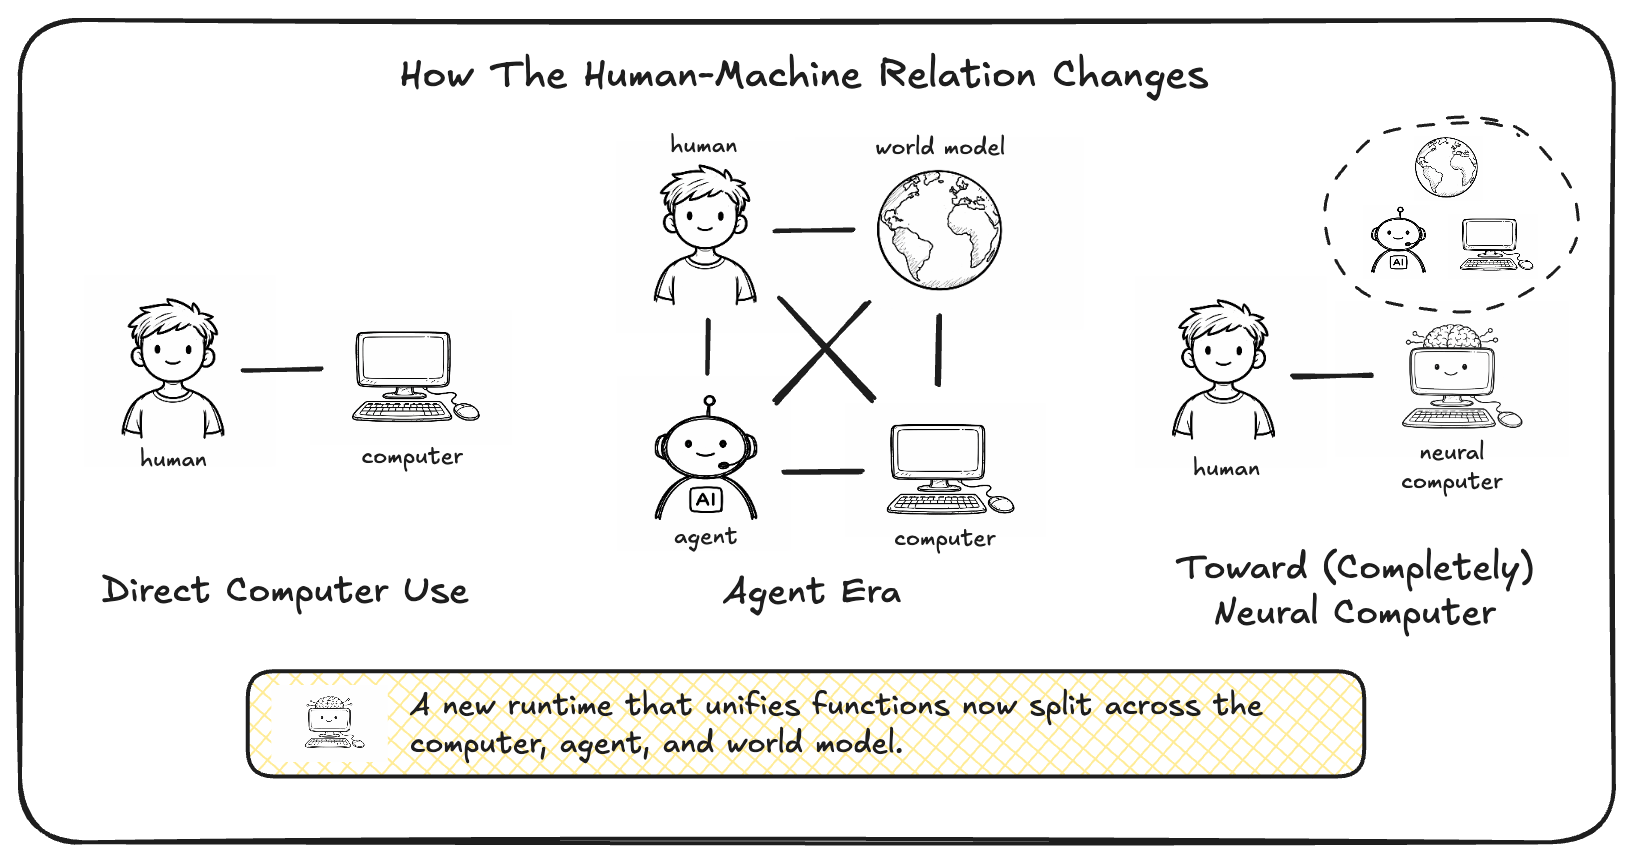
\includegraphics[width=\linewidth]{assets/relations.png}
  \caption{Changing human-machine relations across conventional computers, the agent era, and neural computers. Conventional computers are used directly; in today's agent stack, agents mediate existing computers while world models serve as a parallel predictive layer; NCs aim to unify these split functions within one learned runtime. In this sense, NCs are motivated not by replacing the current stack from the outside, but by internalizing its split functions within one learning machine. A Completely Neural Computer (CNC) is the mature, general-purpose realization of this machine form.}
  \label{fig:relations}
\end{figure}
The comparisons below unpack this shift relative to conventional computers, world models, and AI agents.
\paragraph{Conventional Computers}
Conventional computers remain the reference system object for reliable execution, explicit programmability, and mature governance.
NCs differ not by adding a smarter application layer on top of this substrate, but by shifting computation, memory, and I/O into a learned runtime state.
In this sense, NCs are best viewed as a different candidate machine form and computing substrate rather than as a direct extension of the conventional software stack.
This framing does not imply that conventional computers will disappear soon, but rather that future systems may be built from a different underlying runtime substrate.

\paragraph{World Models}
World models learn environment dynamics by predicting action-conditioned transitions~\citep{ha2018world}.
Such target environments range from the most ambitious, where all sensory inputs form the real world~\citep{schmidhuber1990making}, to much narrower scopes, such as a few control parameters of a robot arm~\citep{feng2023finetuning}.
They provide one technical perspective on current NC prototypes, since interactive computers are an important class of action-conditioned environments, but they do not by themselves define the NC abstraction.
Many current approaches to modeling computational environments, such as the physical world, also rely heavily on computer-generated data~\citep{richter2016playing,tobin2017domain,dosovitskiy2017carla,garcia2023robust}, potentially leading to models that share characteristics with neural computers. 

\paragraph{AI Agents}
Another important comparison point is AI agents built on top of modern AI models and external software substrates, including computer-use agents, coding and multi-agent systems~\citep{openaiComputerUsingAgent,claudeComputerTool,hong2023metagpt,zhuge2024gptswarm_icml,sager2025comprehensivesurveyagentscomputer}, and recursive self-improvement loops~\citep{zhuge2026ai_recursive}. 
These systems place a learned agent between the user and an external execution substrate, whether that substrate is a GUI, a codebase, or a broader software toolchain.
This provides strong leverage from existing computers and software stacks, but it also preserves a strict separation between the learned model and the runtime that actually stores executable state, applies updates, and enforces system contracts.
Computer-use agents operate through low-bandwidth I/O; coding agents typically emit symbolic artifacts that must be executed elsewhere; and RSI-style loops improve the agent by iterating over external tools, prompts, or code rather than by turning the runtime itself into the computer.
Such systems also increasingly rely on automated evaluators, including agent-as-a-judge schemes, to rank outputs, validate task completion, and close iterative improvement loops~\citep{zhuge2024agent_judge}.
We hypothesize that a sufficiently capable NC can internalize many of these agentic functions within one persistent neural runtime.

\subsection{Additional Thoughts} %Inspired by This Research}
The remarks in this section are intended as hypotheses and design directions motivated by the present results, rather than as empirical conclusions established by the current prototypes.

\paragraph{ONE}
ONE~\citep{schmidhuber2018one} proposed a single neural substrate that incrementally absorbs and reuses diverse learned skills. While ONE was not instantiated as a computer-like runtime with explicit I/O, programmability, and update governance, a mature CNC can be viewed as a plausible systems-level realization of this idea. In this sense, many specialized world-model-like components may ultimately appear not as separate external systems, but as installable capabilities within one persistent neural runtime.

\paragraph{Video models as a pragmatic prototype substrate}
We build our prototypes on state-of-the-art video models because they currently provide the simplest path to an end-to-end learned latent runtime state that jointly models pixels, dynamics, and action-conditioned control. This choice is pragmatic rather than fundamental. In our experiments, symbolic and algorithmic reasoning in terminal settings remains inconsistent for most strong video models, and even simple arithmetic can fail (\Cref{tab:cligen-arith}). Sora2 is a notable exception in our probe, achieving $71\%$ arithmetic accuracy, suggesting that some terminal symbolic reasoning is already possible in modern video generators. At the same time, we do not claim that video models cannot reason more broadly: recent work reports that video models can act as zero-shot learners and reasoners in naturalistic settings \citep{wiedemer2025video}. We expect reasoning capabilities to improve quickly with continued progress in video modeling, but our results suggest that CNC-level reliability will likely require additional architectural and training ingredients beyond scaling today's video generators.

\paragraph{A hypothesis: machine-native neural architectures}
We emphasize that the following is a conjecture rather than a conclusion drawn from our experiments. Closing the reasoning gap may not require designing neural networks that more closely mimic animal cognition or the human brain.
Many influential architectures, including convolutional networks \citep{fukushima1980neocognitron} and linear/quadratic Transformers \citep{schmidhuber92fastweights,vaswani2017attention}, are highly engineered systems, but their core inductive biases remain strongly influenced by biological perception and attention. These models primarily rely on continuous, distributed representations, in which reasoning behavior emerges implicitly from large-scale training.
We hypothesize that CNCs may instead benefit from designs that are explicitly machine-native. Developing discrete operations, compositional structures, and verifiable computation that are harmonious in neural systems may play an essential role in designing such systems. This approach follows more closely the construction of conventional computers from well-defined computational primitives and stands in contrast to relying on emergent reasoning in generic video generation models.

\paragraph{Neural networks generation via NC interaction}
Neural network generation can be viewed as a form of programming, i.e., the synthesis of a neural architecture and its corresponding weights. Because NCs' architectural semantics are already neural and numerical, neural components are first-class, and generation directly manipulates the memory state rather than translating it into symbolic code. Moreover, NCs can be programmed through I/O interaction: sequences of inputs, observations, and outcomes act as executable specifications that shape the internal state and routines of the system~\citep{cypher1993watch,myers2002demonstrational}. This suggests a path in which users generate and refine neural modules within NCs through interactive traces, treating interaction logs as programs that configure and compose neural computation.

\paragraph{Unified hardware requirements and data representation}
In NCs, tensors and tensor-to-tensor transformations act as primary computational primitives, replacing the heterogeneous mix of data structures and subsystem-specific abstractions common in conventional computers. Traditional systems span many distinct domains—scalars, pointers, linked structures, files, sockets, and processes—each with its own memory layout, invariants, APIs, and failure modes, coordinated by operating systems through largely disjoint subsystems (virtual memory, filesystems, networking, scheduling, and drivers)~\citep{tanenbaum2013structured,silberschatz2019operating}. Although this heterogeneity supports broad generality, it also fragments optimization and tooling because compilers, profilers, and debuggers must reason across incompatible abstractions~\citep{gregg2014systems}. By contrast, a tensor-uniform pipeline concentrates representation and execution into a compact set of composable primitives, such as linear algebra and elementwise operations, allowing tooling to target a shared intermediate representation~\citep{paszke2019pytorch}. As a result, optimizations such as operator fusion, memory planning, and computational-graph rewriting can be applied system-wide~\citep{vasilache2018tensor}; profiling can focus on throughput and memory bandwidth; and accelerators such as GPUs can be targeted through common tensor runtimes~\citep{sze2017efficient}. This shared numerical representation also naturally supports multimodal computation: vision (pixel tensors), language (sequence embeddings), audio (waveforms or spectrograms), control (state-action tensors), and planning (latent trajectory tensors) all reside in one representational space and can be jointly reasoned over and optimized in a single graph~\citep{ramachandram2017deep}, without repeated type bridging or subsystem translation—steps that are substantially harder in traditional heterogeneous stacks.
